\documentclass{beamer}
\usetheme{Warsaw}
\title{Perl is for pwn!}
\author{Sergey Romanov}
\date{YAPC::Russia 2012}

\begin{document}

\frame{\titlepage}

\frame
{
\frametitle{Hello}
\begin{itemize}
\item Sergey Romanov
\item Do Perl for fun (also, for living)
\item Like alpacas
\end{itemize}
\begin{figure}
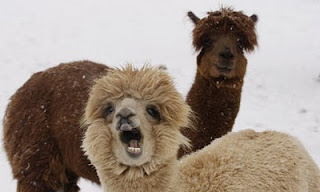
\includegraphics[width=2.5in,height=1.5in]{pics/alpacas.jpg}
\end{figure}
}

\section[CTF]{}

\subsection{What's it all about}
\frame
{
\frametitle{Wiki says that...}
\begin{itemize}
\item Capture the Flag (CTF) is a computer security wargame
\item CTF was popularized by the hacker conference DEFCON
\item Two basic types of competition
\end{itemize}
}

\subsection{Task-based CTF}
\frame
{
\frametitle{Find the key}
\begin{itemize}
\item Teams should solve tasks get points
\item Different categories: web, reverse, packet analysis, admin, ctb (crack-the-box), cryptography etc etc
\item Quals are usually task-based
\end{itemize}
}

\subsection{"Classic" CTF}
\frame
{
\frametitle{Steal the flag}
\begin{figure}
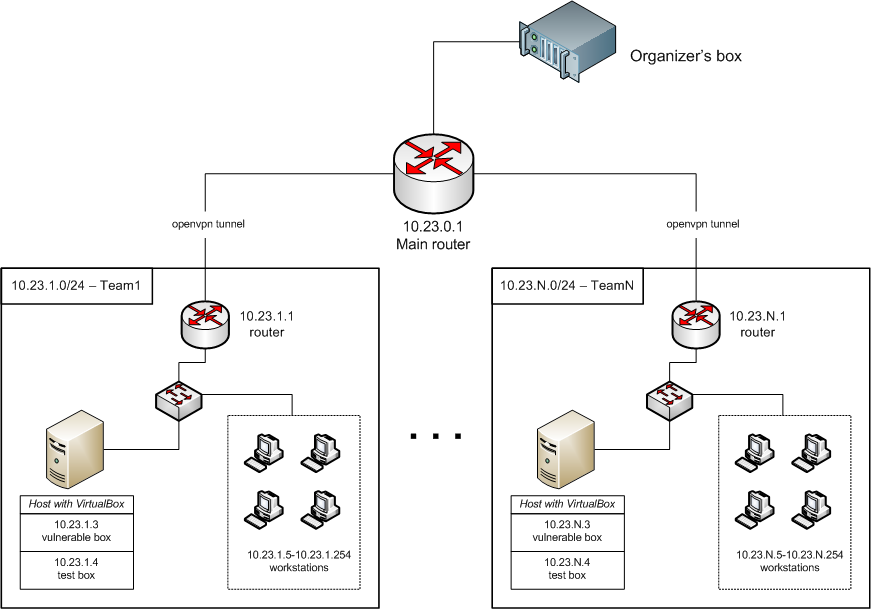
\includegraphics[width=3in,height=2in]{pics/network.png}
\end{figure}
}

\subsection{Okay, we get it}
\frame
{
\frametitle{How about Perl?}
\begin{itemize}
\item<1-> Perl is used during CTF game \_heavily\_
\item<2-> Just like any other modern, popular and convinient tool :)
\item<3-> But we'll concentrate on Perl
\end{itemize}
}

\section{Participant side}

\subsection{Routine tools}
\frame
{
\frametitle{CPAN \& beyond}
\begin{itemize}
\item<1-> /usr/bin/lwp-*
\item<1-> /usr/bin/md5pass
\item<2-> find out yours: \textbf{grep '/usr/bin/perl' /usr/bin/*}
\end{itemize}
}

\frame
{
\frametitle{Gort, Klaatu barada...}
Nikto2
\begin{figure}
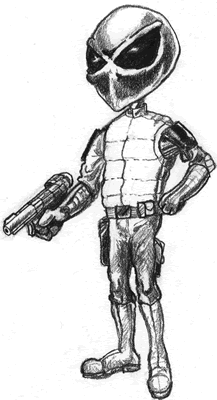
\includegraphics[width=1in,height=2in]{pics/nikto.png}
\end{figure}
}

\frame
{
\frametitle{Nikto2}
\begin{itemize}
\item Web server scanner
\item Based on libwhisker2 by rain forest puppy (rfp)
\item http://cirt.net/nikto2
\end{itemize}
}

\subsection{Flag poster}
\frame
{
\frametitle{Exploitfarm}
\begin{itemize}
\item Written at Hackerdom (USU, Ekaterinburg)
\item Automate process of collecting flags and submitting them to jury check system.
\item http://code.google.com/p/exploitfarm/
\end{itemize}
}

\section{Organizer side}
\subsection{Tasks}
\frame
{
\frametitle{Demo}
}

\subsection{Services}
\frame
{
\frametitle{Demo}
}

\subsection{Check system}
\frame
{
\frametitle{Complex system for CTF-style contests}
\begin{itemize}
\item<1-> Written by Lexi Pimenidis, RWTH Aachen
\item<1-> Gameserver, the Submitserver, and the Scoreserver
\item<1-> Was used at CIPHER, op3n, UralCTF	etc
\item<2-> http://www.cipher-ctf.org/Gameserver.php
\end{itemize}
}

\frame
{
\frametitle{Thank you!}
\begin{figure}

\includegraphics[width=4in,height=2in]{pics/aybabtu.png}
\end{figure}

PS: DEFCON XX Quals start 2 Jun 2012! Join!
}

\end{document}
